\documentclass[a4paper, 20pt]{article}
\usepackage[utf8]{inputenc}
\usepackage{paralist}
\usepackage{jeffe}
\usepackage{handout}
\usepackage{tikz}
\usepackage{gensymb}
\usetikzlibrary{arrows,shapes.gates.logic.US,shapes.gates.logic.IEC,calc}
\usetikzlibrary{positioning}
\usepackage{hyperref}
\usepackage{aurical}
\usepackage[T1]{fontenc}
% definitions for formatting code blocks
\usepackage{listings}

\usepackage{karnaugh-map}

\def\mor{\mathbin{\mid}}
\def\mand{\mathbin{\char`\&}}
\def\rshift{\mathbin{\char`\>\char`\>}}

\def\lnot{\mathop{\sim}}
\def\implies{\mathop{\rightarrow}}
\def\xor{\mathop{\oplus}}

\def\ith#1{${#1}^{\textrm{\scriptsize th}}$}

\begin{document}
\headers{CPSC 121}{ }{Summer 2019}

\begin{center}
    \LARGE
    \textbf{HW 2}
    \\[1ex]
    \Large Due: 23:00, Wednesday May 22, 2019\\
\end{center}
    \LARGE
\begin{tabular}{rl}
 & \\
CS ID 1: &  d6a2b\\
 & \\
CS ID 2: & b9i2b\\
 & \\
\end{tabular}
\large

\textbf{Instructions:}
\begin{enumerate}
\item Do not change the problem statements we are giving you. Simply add your solutions by editing this latex document. 
\item If you need more space, add a page between the existing pages using the \texttt{\textbackslash newpage} command.
\item Include formatting to clearly distinguish your solutions from the given problem text (e.g. use a different font colour for your solutions). Improperly or insufficiently typeset submissions will receive a penalty.
\item Export the completed assignment as a PDF file for upload to Gradescope.
\item On Gradescope, upload only \textbf{one} copy per partnership. (Instructions for uploading to Gradescope are posted on the assignments page of the course website.)
\item Late submissions will be accepted up to 24 hours past the deadline with a penalty of 20\% of the assignment’s maximum value
\end{enumerate}

\textbf{Academic Conduct:} 
I certify that my assignment follows the academic conduct rules for of CPSC 121 as outlined on the course website. As part of those rules, when collaborating with anyone outside my group, (1) I and my collaborators took no record but names away, and (2) after a suitable break, my group created the assignment I am submitting without help from anyone other than the course staff. \\

\textbf{Version history:}
\begin{itemize}
    \item 2019-05-15 00:15 -- Initial version for release
\end{itemize}

\newpage
\begin{question}{1.}
\def\StartsWith#1#2{\textit{Starts}({#1},{#2})}

\item[9] Consider the following sets and predicates: 
  \begin{itemize}
  \item $D$: video game developers
  \item $G$: video game titles
  \item $P$: hardware platforms
  \item $M(d, g)$: developer $d$ made game $g$.
  \item $R(g, p)$: game $g$ released on platform $p$.
  \item $B(d, g)$: developer $d$ bribed a journalist to write a favourable review for game $g$.
  \end{itemize}

  Rewrite each of  the following statements using \textbf{only}  the quantifiers $\forall$
  and $\exists$, the predicates $M$, $R$ and $B$, the domains $D$, $G$, $P$, and $\mathbb{R}$ (the set of real numbers),
  logical connectives, and the operators $=$, $\neq$. $<$, $\le$, $\ge$ and $>$.
  
  If you feel a  sentence is ambiguous, then state your assumed interpretation.
  \begin{question}{a.}[2]

  \item[3] Every developer made a game that released on every platform.
   
   \vspace{2.0in}
   
  \item[3] Some developer bribed a journalist to write a favourable review for a game made by a different developer.
  
  \vspace{2.0in}
   
  \item[3] Some developer bribed journalists to write favourable reviews for every game that the developer made.
  
  \vspace{2.0in}

  \end{question}

\newpage
\\ 1(a).
\\ Proof:
\\ $ \equiv (\lnot p \land (q \rightarrow p)) \rightarrow \lnot q$ [Start]
\\ $ \equiv (\lnot p \land (\lnot q \lor p)) \rightarrow \lnot q$ [IMP]
\\ $ \equiv \lnot (\lnot p \land (\lnot q \lor p)) \lor \lnot q$ [IMP]
\\ $ \equiv ( p \lor \lnot (\lnot q \lor p)) \lor \lnot q$ [IMP]
\\ $ \equiv p \lor \lnot (\lnot q \lor p) \lor \lnot q$ [ASS]
\\ $ \equiv \lnot q \lor p \lor \lnot (\lnot q \lor p) $ [COM]
\\ $ \equiv (\lnot q \lor p) \lor \lnot (\lnot q \lor p) $ [ASS]
\\ $ \equiv T $ [NEG]
\\ \boxed{}
\\ This is a tautology.
\\
\\1(b).
\\Proof:
\\ $\equiv \lnot(a \land b) \rightarrow (b \rightarrow (a \oplus b))$ [Start]
\\ $\equiv (a \land b) \lor (b \rightarrow (a \oplus b))$ [IMP]
\\ $\equiv (a \land b) \lor (\lnot b \lor (a \oplus b))$ [IMP]
\\ $\equiv (a \land b) \lor (\lnot b \lor (\lnot a \land b) \lor (a \land \lnot b))$  [XOR]
\\ $\equiv (a \land b) \lor (\lnot b \lor (a \land \lnot b) \lor (\lnot a \land b))$  [COM]
\\ $\equiv (a \land b) \lor (\lnot b \lor (\lnot a \land b))$  [ABS]
\\ $\equiv (a \land b) \lor (\lnot b \lor \lnot a \land \lnot b \lor b)$ [DIST]
\\ $\equiv (a \land b) \lor (\lnot b \lor \lnot a \land T)$  [NEG]
\\ $\equiv (a \land b) \lor (\lnot b \lor \lnot a)$  [I]
\\ $\equiv (a \land b) \lor \lnot  (a \land b)$  [DM]
\\ $\equiv T$  [NEG]
\\\boxed{}
\\ This is a tautology.
\\
\\ 1(c).
\\ Proof:
\\ $\equiv \lnot c \rightarrow ((\lnot b \rightarrow c)\land (c \rightarrow \lnot a))$ [Start]
\\ $\equiv \lnot c \rightarrow (( b \lor c)\land (c \rightarrow \lnot a))$ [IMP]
\\ $\equiv \lnot c \rightarrow (( b \lor c)\land (\lnot c \lor \lnot a))$ [IMP]
\\ $\equiv c \lor (( b \lor c)\land (\lnot c \lor \lnot a))$ [IMP]
\\ $\equiv (c \lor b \lor c)\land (c \lor \lnot c \lor \lnot a)$ [DIST]
\\ $\equiv (c \lor c \lor b)\land (c \lor \lnot c \lor \lnot a)$ [COM]
\\ $\equiv (c \lor b)\land (c \lor \lnot c \lor \lnot a)$ [ID]
\iffalse
\\ $\equiv (c \lor b)\land (T \lor \lnot a)$ [NEG]
\\ $\equiv (c \lor b)\land \lnot a$ [UB]
\fi
\\\boxed{}
\\ This does not simplify to T. A sample case to prove it's not a tautology is when b is 0 and c is 0. This is not a tautology.
\\
\\ 1(d).
\\ Proof:
\\ $\equiv ((a \land c) \rightarrow (b \rightarrow c)) \land (c \rightarrow a)$ [Start]
\\ $\equiv ((a \land c) \rightarrow (b \rightarrow c)) \land (\lnot c \lor a)$ [IMP]
\iffalse
\\ $\equiv ((a \land c) \rightarrow (\lnot b \lor c)) \land (\lnot c \lor a)$ [IMP]
\\ $\equiv (\lnot (a \land c) \lor (\lnot b \lor c)) \land (\lnot c \lor a)$ [IMP]
\\ $\equiv (\lnot a \lor \lnot c \lor (\lnot b \lor c)) \land (\lnot c \lor a)$ [DM]
\fi
\\ \boxed{}
\\ This does not simplify to T. A sample case to prove it's not a tautology is when a is 0 and c is 1. This is not a tautology.
\\
\newpage
\item[10] Later in the semester we will discover strategies for proving that for integers $a$, $b$, $c$, $d$, and $m$, if $a\equiv b\bmod{m}$ and $c\equiv d\bmod{m}$, then $a\cdot c\equiv b\cdot d\bmod{m}$, and $a+c\equiv b+d\bmod{m}$. In this problem, we will  investigate the meaning of these statements, and see their implications for number representation. Feel free to use a calculator for parts (a), (b), (f), (g), (h), (i) and (l).

\begin{question}{a.}[0.5]
    \item[0.5] Write the 16-bit unsigned representations of 30924.
    \begin{Questions}
    \vfill
    \end{Questions}
    \item[0.5] What is $30924\bmod 32$, expressed in decimal?
    \begin{Questions}
    \vfill
    \end{Questions}
    \item[0.5] Write the 5-bit unsigned representation of your answer to part (b).
    \begin{Questions}
    \vfill
    \end{Questions}
    \item[0.5] Describe the relationship between your answers to parts (a) and (c).
    \begin{Questions}
    \vfill
    \end{Questions}
    \item[1] Explain how you can compute the remainder when 30924 is divided by 16 (in decimal) \emph{in 10 seconds or less}.
    \begin{Questions}
    \vfill\vfill\eject
    \end{Questions}
    \item[0.5] If $a = 30924$, and $b= 48701$, find the least significant 5 bits of $a+b$ (in binary).
    \begin{Questions}
    \vfill
    \end{Questions}
    \item[0.5] Find $30924 \cdot 8\bmod{32}$ (in decimal).
    \begin{Questions}
    \vfill
    \end{Questions}
    \item[1]
    Write the 16-bit two's complement {\em signed} representation of $-30924$.
    \begin{Questions}
    \vfill
    \end{Questions}
    \item[1]
    Find $-30924\mod{32}$ (in binary).
    \begin{Questions}
    \vfill
    \end{Questions}
    \item[1]
    Describe the relationship between your answers to parts (c) and (i).
    \begin{Questions}
    \vfill\vfill
    \end{Questions}
    \item[0.5] If $a = -30924$, and $b= 16653$, find the least significant 5 bits of $a+b$ (in binary).
    \begin{Questions}
    \vfill
    \end{Questions}
    \item[0.5] Find $-30924 \cdot 8\mod{32}$ (in decimal).
    \begin{Questions}
    \vfill\eject
    \end{Questions}
    \item[2]
    By exploration, we have illustrated some of the implications of the simple rules of modular arithmetic. Show that the rule cannot be extended to the division operation, by finding a {\em counter example}. That is, find unsigned integers $a$, $b$, $c$, $d$, and $m$, so that $a\equiv b\mod{m}$ and $c\equiv d\mod{m}$, but $a/c\not\equiv b/d\mod{m}$.
    \begin{Questions}
    \vfill
    \end{Questions}
    
\end{question}
\vfill\eject

\newpage
\\ 2(a).
\\ $30924_1_0 = 0111 1000 1100 1100_2$
\\
\\ 2(b).
\\ 30924 mod 32 = 12
\\
\\ 2(c).
\\ $12_1_0 = 01100_2$
\\
\\ 2(d).
\\ 12 in binary appears in 5 least significant digits of 30924 in binary.
\\
\\ 2(e).
\\ I know that 30924 mod 32 = 12, and 16 is a common denominator of 32, so x mod 32 must output x mod 16, or a number in between 16 to 31. In this case, the answer to 30924 mod 32 = 12, so 30924 mod 16 must also = 12.
\\
\\ 2(f).
\\ $30924_1_0 = 0111 1000 1100 1100_2$
\\ $48701_1_0 = 1011 1110 0011 1101_2$
\\ Adding only the 5 least significant digits:
\\ 01100 + 11101 = 101001
\\ Five least significant digits of a + b in binary is 01001.
\\
\\2(g).
\\ 30924 mod 32 = 12
\\ 8 mod 12 = 8
\\ 12*8 = 96
\\ 96 mod 32 = 0
\\ 30924·8 mod 32 = 0
\\
\\2(h).
\\ $-30924_1_0 = 1000 0111 0011 0100_2$
\\ 
\\ 2(i).
\\ -30924 mod 32 = 20 = $10100_2$
\\
\\ 2(j).
\\ They are both 5 least significant digits of the number that 32 mod into.
\\
\\ 2(k).
\\ $-30924_1_0 = 1000 0111 0011 0100_2$
\\ $16653_1_0 = 0100 0001 0000 1101_2$
\\ Adding only the 5 least significant digits:
\\ 10100 + 01101 = 100001
\\ Five least significant digits of a + b in binary is 00001.
\\
\\2(l).
\\ -30924 mod 32 = 20
\\ 8 mod 12 = 8
\\ 20*8 = 160
\\ 160 mod 32 = 0
\\−30924·8 mod 32 = 0
\\
\\2(m).
\\ 3 = -32 mod 5
\\ 4 = 9 mod 5
\\ -32/9 = -3.556
\\ -3.556 mod 5 = 1.444
\\ 3/4 = 0.75
\\ 1.44 $\neq$ 0.75
\\ Modular operation rule can't extend to division, proven by counter example above.
\newpage
\item[17] Logical Arguments
\begin{question}{a.}[5]

\item[4] Consider the following argument:
\begin{quote}
If there is a chance of rain, or he ate bean chili for lunch, Geoff will not ride his bicycle. Unless Geoff washed his car in the morning, there is no chance of rain. Today Geoff neither washed his car nor ate bean chili. Therefore, Geoff will ride his bicycle today.
\end{quote}

First represent this argument symbolically. Then determine whether it is valid or not.
Justify your answer.
\begin{Questions}
\vfill\eject
\end{Questions}

\item[4] Consider the following argument:
\begin{quote}
If Geoff works hard enough and does not get fired, then he will get paid. If he gets paid, then he will buy food to eat. Geoff has not bought food to eat. Therefore either Geoff did not work hard enough, or he got fired.
\end{quote}

First represent this argument symbolically. Then determine whether it is valid or not.
Justify your answer.
\begin{Questions}
\vfill\eject
\end{Questions}

\item [5]
Consider the following argument:
\begin{quote}
If 30,000 cookies disappeared from Christie's factory, then either Christie destroyed the cookies, or Keebler stole the cookies. If it is not the case that a tree-dwelling elf became the new CEO of Christie and the new Christie CEO colluded with Keebler, then 30,000 cookies disappeared from Christie's factory. If the new Christie CEO did not have a secret meeting with Keebler's industrial spies, then Keebler did not steal the cookies. Christie did not destroy the cookies, and the new Christie CEO had a secret meeting with Keebler's spies. Therefore, Christie's new CEO did not collude with Keebler! No collusion!
\end{quote}

First represent this argument symbolically. Then determine whether it is valid or not.
Justify your answer.
\begin{Questions}
\vfill\eject
\end{Questions}

\item[4]
Determine whether the following argument is valid. If it is valid, show a formal proof and if it is invalid provide a counter-example, i.e. an assignment of truth values that demonstrate a contradiction.


This argument is \underline{~~~~~~~~~~~~~~~~~~~~~}. (Fill in the blank with ``valid'' or ``invalid''.)
\vspace{0.2in}

\hspace{0.4in}\begin{tabular}{r}

$\lnot p \land q$\\
$r \rightarrow p$\\
$\lnot r \rightarrow (s \land t)$\\
$s \rightarrow (t \lor p)$\\
\hline
$\therefore  t  $\\
\end{tabular}
\vspace{0.2in}

Proof:

\hspace{0.4in}\begin{tabular}{r|l}
~~~~~~inference~~~~~~ & rule \\
\hline
 & ~~~~~~~~~~~~~~~~~~~~~~~\\
\hline
 & ~~~~~~~~~~~~~~~~~~~~~~~\\
\hline
 & ~~~~~~~~~~~~~~~~~~~~~~~\\
\hline
 & ~~~~~~~~~~~~~~~~~~~~~~~\\
\hline
 & ~~~~~~~~~~~~~~~~~~~~~~~\\
\hline
 & ~~~~~~~~~~~~~~~~~~~~~~~\\
\hline
 & ~~~~~~~~~~~~~~~~~~~~~~~\\
\hline
 & ~~~~~~~~~~~~~~~~~~~~~~~\\
\hline
 & ~~~~~~~~~~~~~~~~~~~~~~~\\
\hline
 & ~~~~~~~~~~~~~~~~~~~~~~~\\
\hline
 & ~~~~~~~~~~~~~~~~~~~~~~~\\
\hline
 & ~~~~~~~~~~~~~~~~~~~~~~~\\
\hline
 & ~~~~~~~~~~~~~~~~~~~~~~~\\
\hline
 & ~~~~~~~~~~~~~~~~~~~~~~~\\
\hline
 & ~~~~~~~~~~~~~~~~~~~~~~~\\
\hline
\end{tabular}
\large
\vspace{0.2in}

Invalidating truth assignment:\bigskip

$r=~~~~~~$, $s=~~~~~~$, $t=~~~~~~$, $u=~~~~~~$, $w=~~~~~~$


\end{question}
\newpage

\newpage
\\3(a).
\\ a = "There is a chance of rain"
\\ b = "Geoff ate bean chili for lunch"
\\ c = "Geoff will ride his bicycle"
\\ d = "Geoff washed his car in the morning"
\\
\\ Argument:
\\$[1] (a \lor b) \rightarrow \lnot c$
\\$[2] \lnot d \rightarrow \lnot a$
\\$[3] \lnot d \land \lnot b$
\\Therefore [Conclusion] c
\\
\\ Proof:
\\$[5] \lnot (a \lor b) \lor \lnot c$ [IMP 1]
\\$[6] \lnot b$ [SPEC 3]
\\$[7] \lnot d$ [SPEC 3]
\\$[8] \lnot a$ [M.PON 2, 7]
\\$[9] \lnot a \land \lnot b$ [CONJ 6, 8]
\\$[10] a \lor b$ [DM 9]
\\$[11] \lnot c$ [M.PON 1, 10] 
\\\boxed{}
\\
\\ Argument is not valid since premises are true, but conclusion is false.
\\
\\3(b).
\\ a = "Geoff works hard enough"
\\ b = "Geoff gets fired"
\\ c = "Geoff gets paid"
\\ d = "Geoff buys food to eat"
\\
\\Argument:
\\$[1] a \land \lnot b \rightarrow c$
\\$[2] c \rightarrow d$
\\$[3] \lnot d$
\\ Therefore [Conclusion] $\lnot a (+) b$
\\
\\Proof:
\\$[4] a \land \lnot b \rightarrow d$ [TRANS 1, 2]
\\$[5] \lnot (a \land \lnot b)$ [T.MOL 3, 4]
\\$[6] \lnot a \lor b$ [DM 5]
\\ \boxed{}
\\
\\ Argument is invalid since there's at least one truth assignment where all the premises are true but the conclusion is false. A sample one is:
\\ a = 0, b = 1, c = X, d = X
\\
\\3(c).
\\ a = "30,000 cookies disappeared from Christie’s factor"
\\ b = "Christie destroyed the cookie"
\\ c = "Keebler stole the cookie"
\\ d = "a tree-dwelling elf became the new CEO of Christie"
\\ e = "the new Christie CEO colluded with Keebler"
\\ f = "new Christie CEO have a secret meeting with Keebler’s industrial spies"
\\
\\Argument:
\\ $[1] a \rightarrow b \lor c$
\\ $[2] \lnot (d \land e) \rightarrow a$
\\ $[3] \lnot f \rightarrow \lnot c$
\\ $[4] \lnot b$
\\ $[5] f$
\\ Therefore [Conclusion] $\lnot e$
\\
\\ Argument is invalid since there's at least one truth assignment where all the premises are true but the conclusion is false. A sample one is:
\\ a = 1, b = 0, c = 1, d = 0, e = 1, f = 1
\\
\\3(d).
\\This argument is valid.
\\
\\ Argument:\\
$[1]\lnot p \land q$\\
$[2]r \rightarrow p$\\
$[3]\lnot r \rightarrow (s \land t)$\\
$[4]s \rightarrow (t \lor p)$\\
$\therefore [Conclusion] t  $\\
\\ Proof:
\\ $[5] \lnot p$ [SPEC 1]
\\ $[6] \lnot r$ [M.TOL 2,5]
\\ $[7] (s \land t)$ [M.PON 3, 6]
\\ $[8] t$ [SPEC 7]
\\ \boxed{}
\\
\\ Argument is valid because conclusion and premises are true.
\newpage
 \item[8] Using mathematical induction, prove that
 \begin{displaymath}
 \sum_{i=1}^n (i-1) 2^i = (n-2)2^{n+1}
 + 4
 \end{displaymath}
 
 \begin{Questions}
 \\{\color{NavyBlue}
 \\Proof:
 \\
 \\Part 1: Base case
 \begin{gather}
 (n-1) 2^n = (n-2)2^{n+1}+ 4
 \\(1-1) 2^1 = (1-2)2^{1+1}+ 4
 \\0 = 0
 \end{gather}
 \\Part 2: Induction step
 \\
 \\ Assuming that n case is true, we have to prove that this statement is true: 
 \begin{gather}
 \sum_{i=1}^{n+1} (i-1) 2^i = ((n+1)-2)2^{(n+1)+1}+ 4
 \end{gather}
 \\To prove that [4] is true, we say that the sum of n+1 terms is equals to the sum of n terms plus the n+1th term, and simplify from there:
  \begin{gather}
 \sum_{i=1}^{n+1} (i-1) 2^i = \sum_{i=1}^n (i-1) 2^i + ((n+1)-1) 2^{n+1}
 \\ ((n+1)-2)2^{(n+1)+1}+ 4 = ((n-2)2^{n+1}
 + 4) + ((n+1)-1) 2^{n+1}
 \\ (n-1)2^{n+2}+ 4 = (n-2)2^{n+1}
  + n 2^{n+1} + 4
  \\ (n-1)2^{n+2}= (n-2)2^{n+1}
  + n 2^{n+1}
   \\ n2^{n+2} - 2^{n+2} = (n-2)2^{n+1}
  + n 2^{n+1}
   \\ n2^{n+2} - 2^{n+2} = n2^{n+1} - 2^{n+2}
  + n 2^{n+1}
    \\ n2^{n+2} - 2^{n+2} = n2^{n+1} - 2^{n+2}
  + n 2^{n+1}
     \\ n2^{n+2} - 2^{n+2} = 2n2^{n+1} - 2^{n+2}
     \\ n2^{n+2} - 2^{n+2} = n2^{n+2} - 2^{n+2}
 \end{gather}
 \\Steps 5-7 is substituting terms. Step 8 cancels 4 from both sides. Steps 9-10 expands (n-1) and (n-2) terms by distributive property. Steps 11-13 combine like terms to get the final equality. 
 \\Thus, we have proved that when n case is true, n+1 case is true as well. 
 \\}
 \begin{figure}
\begin{verbatim}
         _______                   _____                    _____          
        /::\    \                 /\    \                  /\    \         
       /::::\    \               /::\    \                /::\    \        
      /::::::\    \             /::::\    \              /::::\    \       
     /::::::::\    \           /::::::\    \            /::::::\    \      
    /:::/~~\:::\    \         /:::/\:::\    \          /:::/\:::\    \     
   /:::/    \:::\    \       /:::/__\:::\    \        /:::/  \:::\    \    
  /:::/    / \:::\    \     /::::\   \:::\    \      /:::/    \:::\    \   
 /:::/____/   \:::\____\   /::::::\   \:::\    \    /:::/    / \:::\    \  
|:::|    |     |:::|    | /:::/\:::\   \:::\    \  /:::/    /   \:::\ ___\ 
|:::|____|     |:::|____|/:::/__\:::\   \:::\____\/:::/____/     \:::|    |
 \:::\   _\___/:::/    / \:::\   \:::\   \::/    /\:::\    \     /:::|____|
  \:::\ |::| /:::/    /   \:::\   \:::\   \/____/  \:::\    \   /:::/    / 
   \:::\|::|/:::/    /     \:::\   \:::\    \       \:::\    \ /:::/    /  
    \::::::::::/    /       \:::\   \:::\____\       \:::\    /:::/    /   
     \::::::::/    /         \:::\   \::/    /        \:::\  /:::/    /    
      \::::::/    /           \:::\   \/____/          \:::\/:::/    /     
       \::::/____/             \:::\    \               \::::::/    /      
        |::|    |               \:::\____\               \::::/    /       
        |::|____|                \::/    /                \::/____/        
         ~~                       \/____/                  ~~                  
\end{verbatim}
\caption{A blessed QED to end a blessed proof}
\end{figure}

 \vfill\eject
 \clearpage
 \end{Questions}
 
\newpage
\\4(a).
\\ Assuming carry lower = 1 if result from bits i-1...0 is A < B, and carry greater = 1 if result from bits i-1...0 is A > B. cl and cg can't be both 1 at once, so those values can be considered as don't-care terms. This assumption is in addition to the givens, where $gt=1$ if $A>B$, $eq=1$ if $A=B$, $lt=1$ if $A<B$.
\\
\\
\begin{tabular}{c c c c | c c c}
    $a$ & $b$ & $cl$ & $cg$ & $gt$ & $eq$ & $lt$ \\
    \hline
    0 & 0 & 0 & 0 & 0 & 1 & 0 \\
    0 & 0 & 0 & 1 & 1 & 0 & 0 \\
    0 & 0 & 1 & 0 & 0 & 0 & 1 \\
    0 & 0 & 1 & 1 & X & X & X \\
    \hline
    0 & 1 & 0 & 0 & 0 & 0 & 1 \\
    0 & 1 & 0 & 1 & 0 & 0 & 1 \\
    0 & 1 & 1 & 0 & 0 & 0 & 1 \\
    0 & 1 & 1 & 1 & X & X & X \\
    \hline
    1 & 0 & 0 & 0 & 1 & 0 & 0 \\
    1 & 0 & 0 & 1 & 1 & 0 & 0 \\
    1 & 0 & 1 & 0 & 1 & 0 & 0 \\
    1 & 0 & 1 & 1 & X & X & X \\
    \hline
    1 & 1 & 0 & 0 & 0 & 1 & 0 \\
    1 & 1 & 0 & 1 & 1 & 0 & 0 \\
    1 & 1 & 1 & 0 & 0 & 0 & 1 \\
    1 & 1 & 1 & 1 & X & X & X \\
  \end{tabular}
  
  \\
\\4(b).
\\ Without doing a K-map or a logic simplification, you can just look at it and see that gt and lt is a mux output using a xor b as the selector. When a xor b is 1, gt and lt takes a and b, respectively. When a xor b is 0, gt and lt takes cg and cl, respectively. We can use mux equivalence in logic gates to wire up gt and lt. eq is just a simple sum of minterms. 
\\
 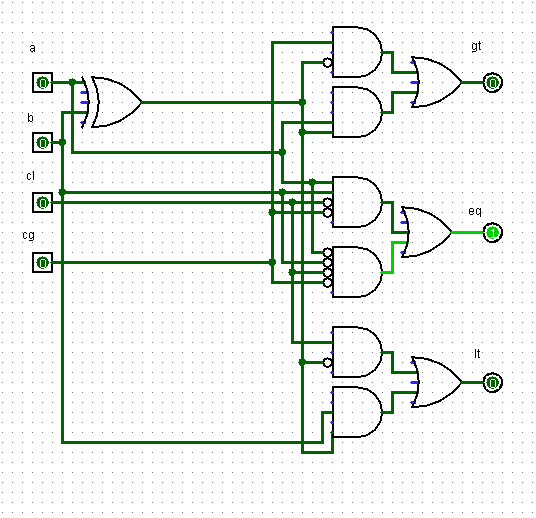
\includegraphics[height=10cm]{4b.png} \\
 \\
\\ 4(c).
\\ It's connecting the 4 corresponding bits of A and B to each comparator, and connecting gt and lt of comparator i-1 to cg and cl of comparator i. cg and cl of comparator 0 should be grounded since it's the first digit / no carry yet. Final output is hooked to the 4th comparator (comparator 3). You can keep adding comparators to make your input however many digits you'd like.
\\
 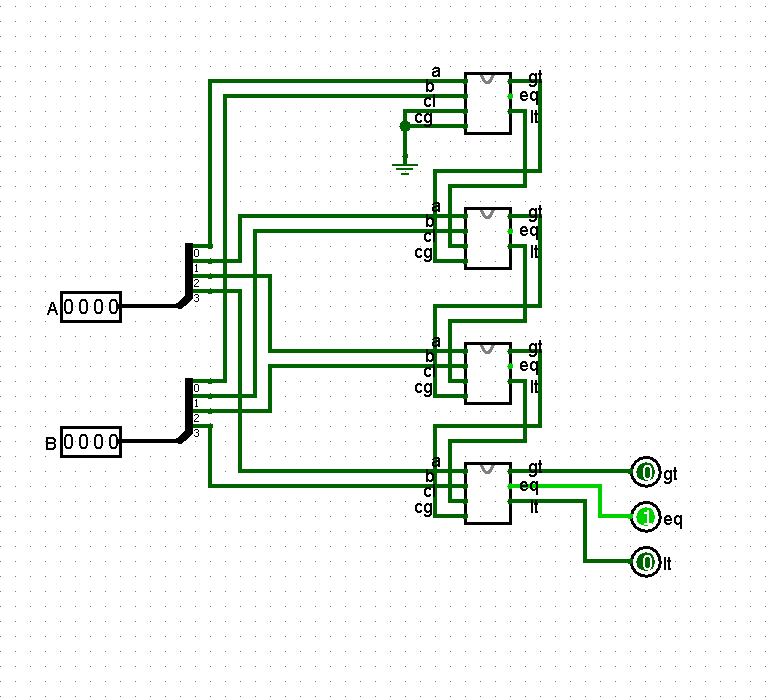
\includegraphics[height=12cm]{4c.png} \\
\newpage
\end{question}
\end{document}
